\section{Kanalcodierung}
\subsection{Blockcodes}
Ein (n,k)-Blockcode wird generiert mit $k$ Eingangssymbolen und $n$ Ausgangssymbolen (n $\gt$ k). Bsp. handelt es sich bei RS232-Übertragung mit 8 Daten- und 1 Paritätsbit um ein (9, 8)-Blockcode.~\\

\noindent Die \textbf{Coderate} $R_C = \frac{k}{n}$~\\

\subsubsection{Operationen}
Module-2-Addition Operation $\oplus$ entspricht einem logischen XOR ($[0,0] = 0; [1,0] = 1; [0,1] = 1; [1,1] = 0)$ und die Multiplikation $\cdot$ einem logischen AND.

\subsection{Lineare Blockcodes}\script{216}
Ein Code giltet als linear, falls jedes beliebigen Codewortes $\vec{a} \oplus \vec{b} = \vec{c}$ wiederum ein Codewort ist. 
\[
\vec{c} = \vec{a}\oplus\vec{b} = \left(a_1 \oplus b_1, \dots a_n \oplus b_n\right)
\]
Weil $\vec{a}\oplus\vec{a} = \vec{0}$, gilt zwingend, dass zu jedem linearen Code der Nullvektor $\vec{0}$ dazu gehört! Zudem ist jeder Code, der mit einer Generatormatrix gebildet werden kann ein linearer Code.

\subsection{Hamming}\script{217}
\noindent Das \textbf{Hamming-Gewicht} $w\vec{c}$ eine Codewortes $\vec{c}$ entspricht der Anzahl Elemente, welche im Codevektor ungleich Null sind. \[w(\vec{c}) = d(\vec{c}, \vec{0})\]

\noindent Die \textbf{Hamming-Distanz} $d(\vec{a}, \vec{b})$ zweier Codeworte $\vec{a}$ und $\vec{b}$ entspricht der Anzahl unterschiedlichen Stellen. \[d = w(\vec{a} \oplus \vec{b})\]

\noindent Die \textbf{Minimale Hamming-Distanz} $d_{min}$ entspricht also dem kleinsten Gewicht eines Codewortes $\vec{c} \neq \vec{0}$. Dies kann auch mit Paritätsprüfmatrix berechnet werden~\\

\noindent Die \textbf{Hamming-Schranke} \script{222} stellt sicher, dass Fehler mit Sicherheit korrigiert werden können. Dabei ist $t$ die korrigierbaren Fehler (Siehe Kapitel \ref{fehlererkennung}) und (n,k)-Blockcode vom Blockcode.
\[
2^{n-k} \ge \sum_{i=0}^{t_c}\begin{pmatrix}
	n \\ i
\end{pmatrix}
\]
Gilt für ein Code das Gleichheitszeichen, handelt es sich um einen perfekten Code.

\subsection{Fehlererkennung}\script{218}\label{fehlererkennung}
Durch die minimale Hamming-Distanz $d_{min}$ ist die Anzahl korrigierbarer und detektierbarer Fehler gegeben:
\begin{itemize}[nosep]
	\item Anzahl \textbf{detektierbarer} Fehler $t_d = d_{min} - 1$
	\item Anzahl \textbf{korrigierbarer} Fehler $t_c =\lfloor \frac{d_{min} - 1}{2}\rfloor$
\end{itemize}

\subsection{Systematische Blockcodes}
\script{128} Ein Blockcode $C$ bezeichnet man als systematisch, falls Elemente des ursprünglichen Datenvektors $d$ an ausgewählter Positioen des Codewortes $c$ wiederzufinden sind.

\subsubsection{Generator Matrix}
Die Generatormatrix $\mathbf{G}$ generiert ein gültiges Codewort $c$ aus dem Datenwort $d$.
\[
\vec{c} = \vec{d} \cdot \mathbf{G}
\]
Dabei ist die Generatormatrix zusammengesetzt aus Paritätsmatrix $P$ und der Einheitsmatrix $I$: $\mathbf{G} = [ \mathbf{I} \mathbf{P}^T ]$. Daraus kann zudem die \textbf{Bildungsgleichung} erstellt werden. (Siehe \script{224} für Beispiel)


\subsubsection{Auswertung}
Das Fehlersyndrom $s$ erlaubt die Erkennung und eventuelle Korrektur von Übertragungsfehlern. Angenommen das empfangene Codewort $c_r$ ist mit einem Fehler $e$ versehen.
\[
\vec{s} = \vec{e} \cdot \mathbf{H}^T
\]
\begin{itemize}[nosep]
	\item $\vec{s} = 0$: kein Fehler erkannt
	\item $\vec{s} \in \mathbf{H}^T$: Fehler erkannt und $i$-te Zeile muss korrigiert werden
	\item Sonst Linearkombinationen (Siehe auch \script{222} \textbf{Restfehlerwahr.keit})
\end{itemize}


\subsection{Zyklische Blockcodes}
\script{227} Coder und Decoder sind aber einer gewissen Blockgrösse aufwendig zu realisieren, abhilfe schaffen die zyklischen Blockcodes:
\begin{align*}
	\sigma(\vec{c}) &= \vec{c}^{(1)} = \left(c_{n-1}, c_0, c_1, \cdots, c_{n-2}\right) \\	
	\sigma^2(\vec{c}) &= \vec{c}^{(2)} = \left(c_{n-2}, c_{n-1}, c_1, \cdots, c_{n-3}\right)
\end{align*}

Wenn die zyklische Verschiebung $\sigma(\vec{c})$ wieder ein gültiges Codewort ergibt, so handelt es sich um einen linearen Blockcode.

\subsection{Polynomdarstellung}
Eine weitere Darstellung für zyklische Blockcodes:
\[
\vec{c} = \left(c_0, c_1, \cdots, c_{n-1}\right) \xrightarrow{} c(x) = c_0 + c_1x + \cdots + c_{n-1}x^{n-1}
\]
Solche Polynome können nun Module-2-Addition addiert werden und somit $1 \oplus 1 = 0$ bzw $x^i \oplus x^i = 0$ gilt. \textbf{Addition und Subtraktion} sind zudem identisch:
\begin{align*}
	\vec{a} &= [110011] = 1 + x + x^4 +x^5 \\
	\vec{b} &= [010101] = x + x^3 + x^5 \\
	\vec{a} + \vec{b} &= [100110] = 1 + x^3 + x^4
\end{align*}

\textbf{Multiplikation} \script{228} schriftlich ausmultiplizieren und Module-2-Addieren 
Beispiel: $(1 + x + x^4 +x^5)\cdot(x+x^3+x^5)$~\\~\\
\begin{tabular}{lllllllllll|l}
	0 & 1 & 2 & 3 & 4 & 5 & 6 & 7 & 8 & 9 & 10 &\\ \toprule
& $x$ & & $x^3$ & & $x^5$ &&&& & & $\oplus$ \\
&& $x^2$ && $x^4$ && $x^6$ &&&& & $\oplus$\\
&&&&& $x^5$ && $x^7$ && $x^9$ & & $\oplus$\\
&&&&&& $x^6$ && $x^8$ && $x^{10}$ & $\oplus$\\ \midrule
& $x$ & $x^2$ & $x^3$ & $x^4$ &&& $x^7$ & $x^8$ & $x^9$ & $x^{10}$
\end{tabular}
Was zu einem Endergebniss von $[01111001111]$ führt.

\textbf{Division} \script{229} von $f$ durch $h$ ist eine spezieller Operation, da der Quotient $q$ mit Rest $r$ addiert werden muss:
\[
\frac{f}{h} = q + \frac{r}{h} \xrightarrow{} f = q\cdot h + r
\]
Um $q$ und $r$ zu berechnen muss die übliche Polynomdivision angewendet werden, jedoch bei Addition und Subtraktion immer $\oplus$ rechnen.


\subsection{Generator Polynom $g(x)$}
Jeder [n,k] zyklische Code kann mit Hilfe des Generator-Polynom $g(x)$ vom Grad $m =n-k$ durch Multiplikation mit dem Daten-Polynom $d$ gebildet werden.
\[
c(x) = d(x) \cdot g(x)
\]

\subsection{Syndrom-Polynom $s(x)$}
Das Fehlersyndrom $s$ from Grad $m=n-k$ dient zur Ermittlung von Übertragungsfehlern. Entählt das empfangene Codewort $c_r$ ein Fehlermuster $e$, so entspricht der Rest der Division (Modulo) dem sog Fehlersyndrom $s$. Ist $s=0$ ist kein Fehler aufgetreten. Mihilfe von $s$ kann das erhaltene Codewort $c_r$ korrigiert werden, wenn $t_c$ kleiner ist (Siehe Kapitel \ref{fehlererkennung})!
\[
s(x) = c_r(x) \mod g(x)
\]

\subsection{Realisierung}
Dabei werden die Generator-Elemente sortiert und anschliessend beschriftet. \textbf{Beispiel} (n=23,k=12)-Blockcode
\begin{align*}
	 1 &+ x + x^5 +x^6 + x^7 + x^9 + x^{11}\\
	\rightarrow \quad g_0 &+ g_1 + g_5 + g_6 +g_7 + g_9 + g_{11}
\end{align*}
\begin{center}
	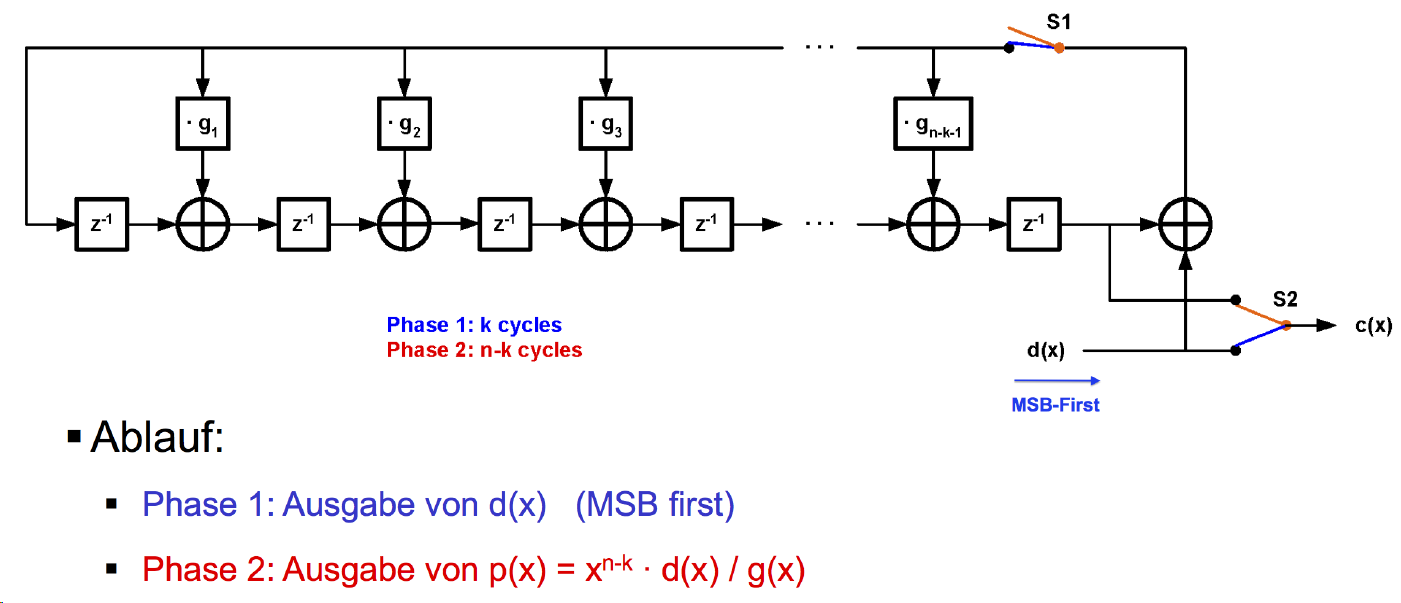
\includegraphics[width=\columnwidth]{Images/realisierung}
\end{center}
